\section{Random Forest}\label{sec:rf}

\subsection{Giới thiệu về Random Forest}
Random Forest \cite{breiman2001} là thuật toán \textit{ensemble} theo hướng \textit{bagging}: huấn luyện $T$ cây quyết định, mỗi cây trên một mẫu bootstrap (lấy ngẫu nhiên có hoàn lại) của tập huấn luyện, và tại mỗi nút chỉ xét một tập con ngẫu nhiên gồm \texttt{max\_features} đặc trưng. Xác suất rời bỏ là trung bình xác suất của các cây. Nếu mỗi cây có phương sai $\sigma^2$ và tương quan giữa hai cây là $\rho$:
\begin{equation}
    \hat{p}(\mathbf{x}) = \frac{1}{T} \sum_{t=1}^{T} \hat{p}_t(\mathbf{x}), \qquad
    \operatorname{Var}\left[\hat{p}(\mathbf{x})\right] = \rho \sigma^2 + \frac{1 - \rho}{T} \sigma^2
\end{equation}
Tăng số cây làm giảm số hạng thứ hai, còn việc chọn ngẫu nhiên đặc trưng làm giảm $\rho$; nhờ vậy Random Forest giảm phương sai cao của cây đơn mà không tăng nhiều độ chệch.

\begin{figure}[H]
\centering
\begin{tikzpicture}[
    node distance=0.5cm and 1.2cm,
    box/.style={rectangle, rounded corners, draw=black!60, minimum height=0.7cm, minimum width=2cm, align=center, font=\small},
    arrow/.style={-{Stealth[length=2mm]}, thick}
]
\node[box, fill=orange!15] (data) {Tập huấn luyện $\mathcal{D}$};
\node[box, fill=yellow!20, below left=of data, xshift=-0.4cm] (b1) {Bootstrap $\mathcal{D}_1$ $\rightarrow$ Cây $h_1$};
\node[box, fill=yellow!20, below=of data] (b2) {Bootstrap $\mathcal{D}_2$ $\rightarrow$ Cây $h_2$};
\node[box, fill=yellow!20, below right=of data, xshift=0.4cm] (bT) {Bootstrap $\mathcal{D}_T$ $\rightarrow$ Cây $h_T$};
\node[box, fill=green!12, below=0.9cm of b2] (avg) {Trung bình xác suất $\hat{p}(\mathbf{x})$; rời bỏ nếu $\hat{p}(\mathbf{x}) > t$};
\draw[arrow] (data) -- (b1); \draw[arrow] (data) -- (b2); \draw[arrow] (data) -- (bT);
\draw[arrow] (b1) -- (avg); \draw[arrow] (b2) -- (avg); \draw[arrow] (bT) -- (avg);
\end{tikzpicture}
\caption{Kiến trúc tổng quát của Random Forest ($t$: ngưỡng quyết định)}
\end{figure}

\begin{table}[H]
\centering
\begin{adjustbox}{max width=\textwidth}
\begin{tabular}{|p{7cm}|p{7cm}|}
\hline
\textbf{Ưu điểm} & \textbf{Nhược điểm} \\
\hline
Chính xác, ổn định; giảm phương sai so với cây đơn & Tốn bộ nhớ và thời gian khi nhiều cây \\
\hline
Không cần chuẩn hóa, tự học tương tác phi tuyến & Khó diễn giải hơn cây đơn \\
\hline
Hỗ trợ class weight và feature importance & Impurity importance thiên vị đặc trưng nhiều giá trị \\
\hline
\end{tabular}
\end{adjustbox}
\caption{Ưu và nhược điểm của Random Forest}
\end{table}

\subsection{Mã nguồn và huấn luyện}
\begin{lstlisting}[style=pythonstyle, caption={Khởi tạo Random Forest trong \texttt{src/models.py}}]
if model_name == "random_forest":
    return RandomForestClassifier(
        n_estimators=100,
        class_weight=class_weight,   # "balanced" khi dung class weight
        random_state=random_state,
        n_jobs=1,
    )
\end{lstlisting}

\texttt{RandomizedSearchCV} (không gian tìm kiếm ở Mục~\ref{sec:exp4}) thử 40 tổ hợp trên 5 fold, chọn theo PR-AUC. Cấu hình tốt nhất: 287 cây, \texttt{max\_depth=8}, \texttt{max\_features=0,5} (mỗi nút xét một nửa số cột), \texttt{min\_samples\_leaf=11}.

\subsection{Kết quả và đánh giá}

\subsubsection{Kết quả cross-validation qua các giai đoạn}
\begin{table}[H]
\centering
\small
\begin{adjustbox}{max width=\textwidth}
\begin{tabular}{|l|c|c|c|c|c|c|}
\hline
\textbf{Cấu hình} & \textbf{Precision} & \textbf{Recall} & \textbf{F1} & \textbf{ROC-AUC} & \textbf{PR-AUC} & \textbf{F1 train} \\
\hline
Baseline (100 cây) & 0,628 & 0,480 & 0,544 & 0,820 & 0,610 & 0,997 \\
\hline
+ Class weight & 0,563 & 0,638 & 0,598 & 0,822 & 0,604 & 0,988 \\
\hline
+ Tuning & 0,531 & 0,776 & 0,631 & 0,848 & 0,667 & 0,699 \\
\hline
+ Ngưỡng 0,60 (out-of-fold) & 0,591 & 0,695 & \textbf{0,639} & 0,848 & 0,667 & -- \\
\hline
\end{tabular}
\end{adjustbox}
\caption{Random Forest: kết quả validation (trung bình 5 fold) qua từng bước}
\end{table}

Ở cấu hình mặc định, Random Forest đã giảm được phương sai so với cây đơn (ROC-AUC 0,820 so với 0,654) nhưng từng cây vẫn học thuộc tập huấn luyện (F1 train 0,997). Class weight tăng F1 thêm 0,054; tuning tiếp tục tăng F1 0,033 và PR-AUC 0,063 (cải thiện ở cả 5 fold), đồng thời thu hẹp khoảng cách F1 train--validation từ 0,39 xuống 0,07.

\subsubsection{Kết quả trên tập test}
\begin{table}[H]
\centering
\begin{minipage}[t]{0.56\textwidth}
\centering
\small
\begin{adjustbox}{max width=\textwidth}
\begin{tabular}{|l|c|c|c|c|}
\hline
\textbf{Lớp} & \textbf{Precision} & \textbf{Recall} & \textbf{F1-score} & \textbf{Support} \\
\hline
Không rời bỏ (0) & 0,88 & 0,81 & 0,84 & 1.035 \\
\hline
Rời bỏ (1) & 0,57 & 0,70 & 0,62 & 374 \\
\hline
Accuracy & & & 0,78 & 1.409 \\
\hline
Macro avg & 0,72 & 0,75 & 0,73 & 1.409 \\
\hline
Weighted avg & 0,80 & 0,78 & 0,78 & 1.409 \\
\hline
\end{tabular}
\end{adjustbox}
\caption{Random Forest: kết quả phân loại trên tập test (ngưỡng 0,60; ROC-AUC 0,843; PR-AUC 0,651)}
\end{minipage}\hfill
\begin{minipage}[t]{0.42\textwidth}
\centering
\small
\begin{adjustbox}{max width=\textwidth}
\begin{tabular}{|c|c|c|c|}
\cline{3-4}
\multicolumn{2}{c|}{} & \multicolumn{2}{c|}{\textbf{Dự đoán}} \\
\cline{3-4}
\multicolumn{2}{c|}{} & Không rời bỏ & Rời bỏ \\
\hline
\multirow{2}{*}{\textbf{Thực tế}} & Không rời bỏ & \cellcolor{blue!30}836 & 199 \\
\cline{2-4}
 & Rời bỏ & 114 & \cellcolor{blue!30}260 \\
\hline
\end{tabular}
\end{adjustbox}
\caption{Random Forest: Confusion Matrix trên tập test}
\end{minipage}
\end{table}

Random Forest có Precision lớp rời bỏ (0,566) và Accuracy (0,778) cao nhất trong bốn mô hình, với ít cảnh báo nhầm nhất (199). Đáng chú ý, trên tập test F1 ở ngưỡng 0,5 (0,639) cao hơn ở ngưỡng đã chọn 0,60 (0,624): ngưỡng tối ưu trên tập train không chuyển tốt sang tập test với mô hình này. So với lần đánh giá test đầu tiên (tham số mặc định, ngưỡng 0,5), F1 tăng từ 0,544 lên 0,624 và Recall từ 0,481 lên 0,695.

\subsubsection{Feature Importance}
\begin{figure}[H]
\centering
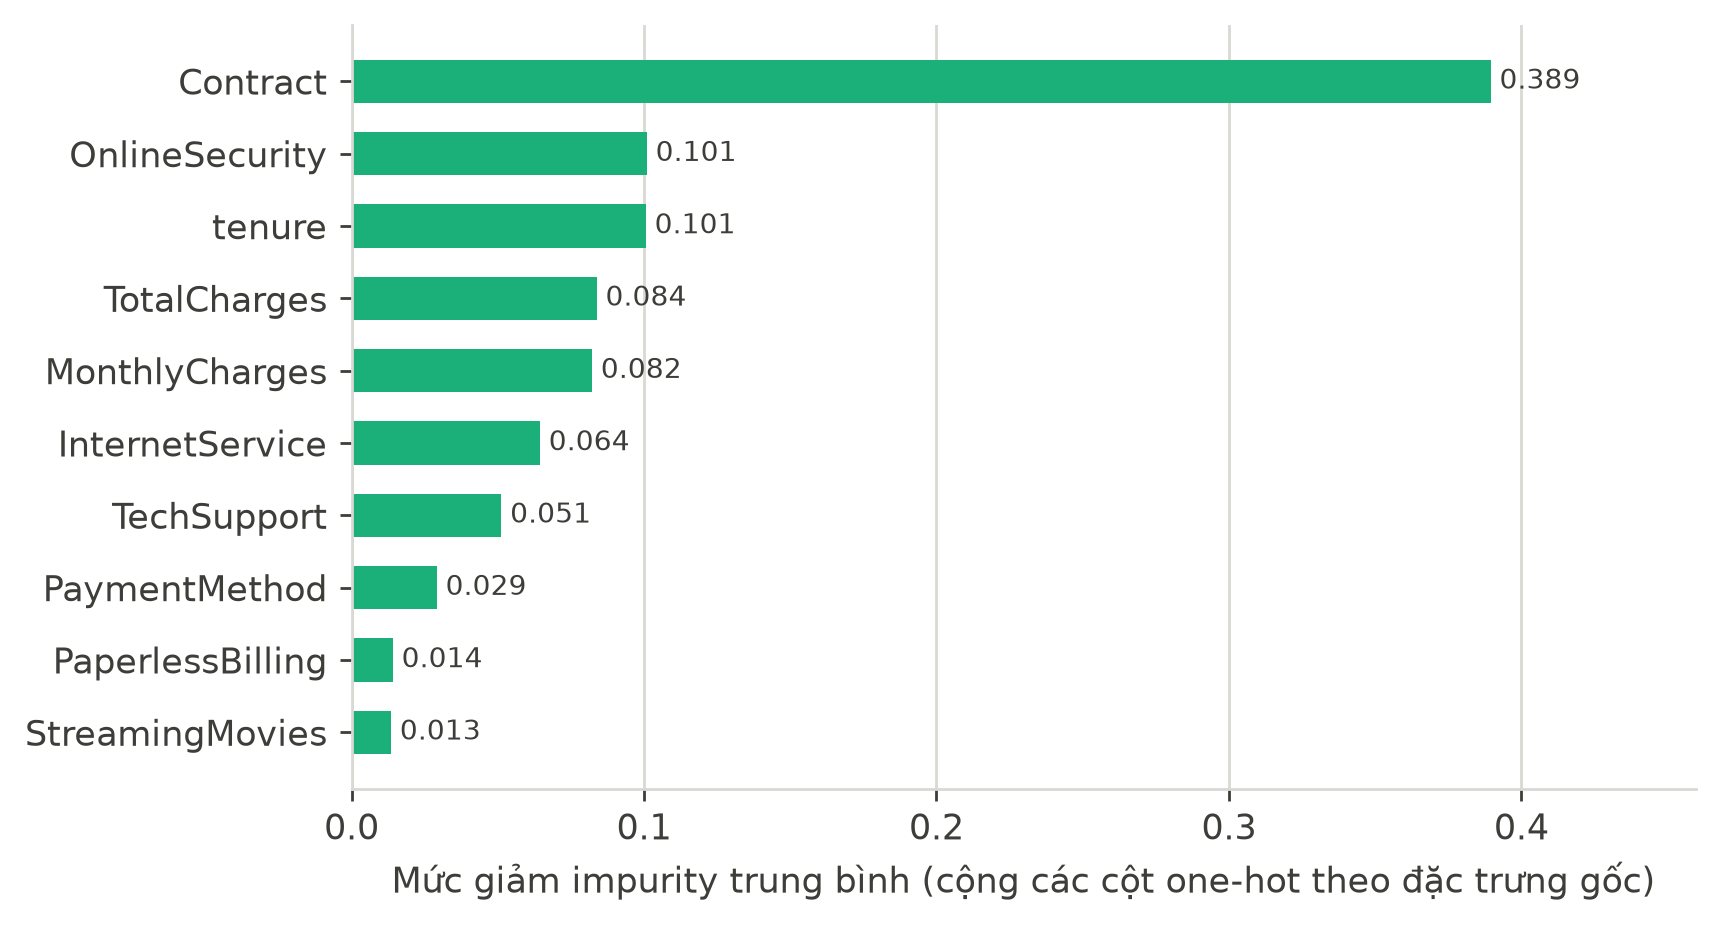
\includegraphics[width=0.75\textwidth]{img/importance_random_forest.png}
\caption{Random Forest: impurity importance của 10 đặc trưng gốc quan trọng nhất}
\end{figure}

\texttt{Contract} vẫn là đặc trưng quan trọng nhất (39\%) nhưng tỉ trọng thấp hơn ở Decision Tree (52\%): nhờ \texttt{max\_features=0,5}, nhiều cây không được xét \texttt{Contract} ở nút gốc và phải dùng các đặc trưng khác. Tiếp theo là \texttt{OnlineSecurity} và \texttt{tenure} (mỗi đặc trưng 10\%), \texttt{TotalCharges} và \texttt{MonthlyCharges} (8\%), \texttt{InternetService} (6\%) và \texttt{TechSupport} (5\%).

\subsubsection{Nhận xét và đánh giá}
\textbf{Điểm mạnh}
\begin{itemize}
    \item PR-AUC cross-validation cao thứ hai (0,667), chỉ kém XGBoost 0,004 -- nhỏ hơn độ lệch chuẩn giữa các fold.
    \item Precision và Accuracy cao nhất trên tập test, ít cảnh báo nhầm nhất: phù hợp khi nguồn lực chăm sóc khách hàng hạn chế.
    \item Ổn định nhờ trung bình hóa nhiều cây; không cần chuẩn hóa đặc trưng.
\end{itemize}

\textbf{Hạn chế}
\begin{itemize}
    \item Khoảng cách F1 train--validation sau tuning vẫn lớn nhất trong bốn mô hình (0,07).
    \item Mô hình cồng kềnh nhất: 287 cây sâu tới 8 tầng, file mô hình khoảng 5,7 MB so với dưới 0,4 MB của ba mô hình còn lại.
    \item Khó diễn giải từng dự đoán; impurity importance thiên vị các đặc trưng số có nhiều điểm chia.
\end{itemize}

\textbf{Hướng cải thiện}
\begin{enumerate}
    \item Chọn ngưỡng ổn định hơn, ví dụ lấy trung vị ngưỡng tối ưu của từng fold, vì ngưỡng 0,60 không chuyển tốt sang tập test.
    \item Thử \texttt{ExtraTreesClassifier} hoặc tăng \texttt{min\_samples\_leaf} để giảm thêm overfitting.
\end{enumerate}
